\documentclass[../../full]{subfiles}


\begin{document}
    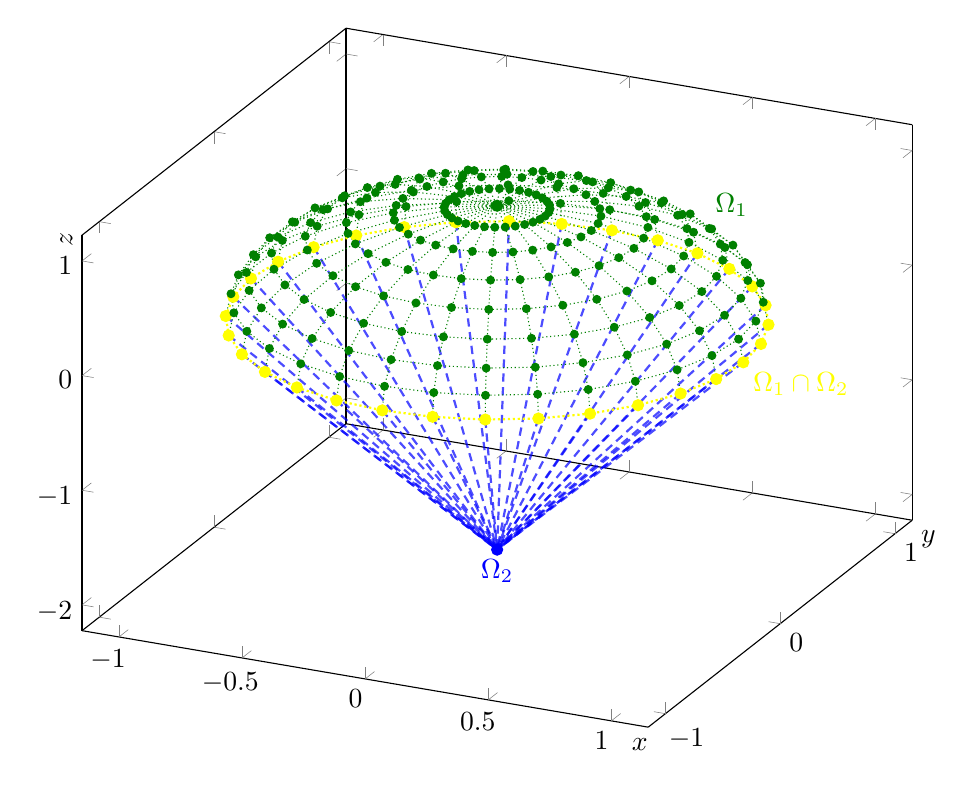
\begin{tikzpicture}
        % colors
        \def\ColorOne{Green}
        \def\ColorTwo{Blue}
        \def\ColorMix{Yellow}
        % angles
        \def\AnglePartsQuart{8}
        \pgfmathtruncatemacro\AnglePartsQuartLess{\AnglePartsQuart-1}
        \pgfmathtruncatemacro\AnglePartsFull{4*\AnglePartsQuart}
        %
        \begin{axis}[
            width=\textwidth,
            view={25}{30},
            xlabel={\( x \)},
            ylabel={\( y \)},
            zlabel={\( z \)},
            xmin=-1, xmax=1,
            ymin=-1, ymax=1,
            zmin=-2, zmax=1,
            enlargelimits=0.075,
            every axis x label/.append style={at=(ticklabel* cs:1)},
            every axis y label/.append style={at=(ticklabel* cs:1)},
            every axis z label/.append style={at=(ticklabel* cs:1)},
        ]
            % marks
            \addplot3 [only marks, \ColorOne] coordinates {(0, 0, 1)};
            \foreach \i [
                    evaluate=\i as \AngleH
                                using (360/\AnglePartsFull*\i),
                    evaluate=\AngleH as \Hx using cos(\AngleH),
                    evaluate=\AngleH as \Hy using sin(\AngleH),
            ] in {1, ..., \AnglePartsFull} {
                \edef\temp{
                    \noexpand \addplot3
                        [\ColorMix, only marks]
                        coordinates { (\Hx, \Hy, 0) };
                }
                \temp
            }
            \addplot3 [only marks, \ColorTwo] coordinates {(0, 0, -2)};
            % Area Two
            \foreach \i [
                    evaluate=\i as \AngleH
                                using (360/\AnglePartsFull*\i),
                    evaluate=\AngleH as \Hx using cos(\AngleH),
                    evaluate=\AngleH as \Hy using sin(\AngleH),
            ] in {1, ..., \AnglePartsFull} {
                \edef\temp{
                    \noexpand \addplot3
                        [
                            \ColorTwo,
                            no marks,
                            thick, densely dashed,
                            opacity=0.7
                        ]
                        coordinates { (\Hx, \Hy, 0) (0, 0, -2) };
                }
                \temp
            }
            % Area Overlap
            \def\TempPath{}
            \foreach \i [
                    evaluate=\i as \AngleH
                                using (360/\AnglePartsFull*\i),
                    evaluate=\AngleH as \Hx using cos(\AngleH),
                    evaluate=\AngleH as \Hy using sin(\AngleH),
                    evaluate=\AngleH as \Px using (\Hx),
                    evaluate=\AngleH as \Py using (\Hy),
                    evaluate=\AngleH as \Pz using (0),
            ] in {0, ..., \AnglePartsFull} {
                \global\edef\TempPath{\TempPath (\Px, \Py, \Pz)}
            }
            \addplot3 [\ColorMix, no marks, thick, densely dotted]
                coordinates {\TempPath};
            % Area One
            \foreach \i [
                    evaluate=\i as \AngleH
                                using (360/\AnglePartsFull*\i),
                    evaluate=\AngleH as \Hx using cos(\AngleH),
                    evaluate=\AngleH as \Hy using sin(\AngleH),
            ] in {1, ..., \AnglePartsFull} {
                \foreach \j [
                        evaluate=\j as \AngleV
                                    using (90/\AnglePartsQuart*\j),
                        evaluate=\AngleV as \Vx using cos(\AngleV),
                        evaluate=\AngleV as \Vy using sin(\AngleV),
                        evaluate=\AngleV as \Px using (\Vx*\Hx),
                        evaluate=\AngleV as \Py using (\Vx*\Hy),
                        evaluate=\AngleV as \Pz using (\Vy),
                ] in {1, ..., \AnglePartsQuartLess} {
                    \edef\temp{
                        \noexpand \addplot3
                            [
                                \ColorOne,
                                only marks, mark options={scale=0.7}
                            ]
                            coordinates {(\Px, \Py, \Pz)};
                    }
                    \temp
                }
                \def\TempPath{}
                \foreach \j [
                        evaluate=\j as \AngleV
                                    using (90/\AnglePartsQuart*\j),
                        evaluate=\AngleV as \Vx using cos(\AngleV),
                        evaluate=\AngleV as \Vy using sin(\AngleV),
                        evaluate=\AngleV as \Px using (\Vx*\Hx),
                        evaluate=\AngleV as \Py using (\Vx*\Hy),
                        evaluate=\AngleV as \Pz using (\Vy),
                ] in {0, ..., \AnglePartsQuart} {
                    \global\edef\TempPath{\TempPath (\Px, \Py, \Pz)}
                }
                \edef\temp{
                    \noexpand \addplot3
                        [\ColorOne, no marks, thin, densely dotted]
                        coordinates {\TempPath};
                }
                \temp
            }
            \foreach \j [
                    evaluate=\j as \AngleV
                                using (90/\AnglePartsQuart*\j),
                    evaluate=\AngleV as \Vx using cos(\AngleV),
                    evaluate=\AngleV as \Vy using sin(\AngleV),
            ] in {1, ..., \AnglePartsQuartLess} {
                \def\TempPath{}
                \foreach \i [
                        evaluate=\i as \AngleH
                                    using (360/\AnglePartsFull*\i),
                        evaluate=\AngleH as \Hx using cos(\AngleH),
                        evaluate=\AngleH as \Hy using sin(\AngleH),
                        evaluate=\AngleV as \Px using (\Vx*\Hx),
                        evaluate=\AngleV as \Py using (\Vx*\Hy),
                        evaluate=\AngleV as \Pz using (\Vy),
                ] in {0, ..., \AnglePartsFull} {
                    \global\edef\TempPath{\TempPath (\Px, \Py, \Pz)}
                }
                \edef\temp{
                    \noexpand \addplot3
                        [\ColorOne, no marks, thin, densely dotted]
                        coordinates {\TempPath};
                }
                \temp
            }
            % labels
            \node [below] at (axis cs: 0, 0, -2)
                [\ColorTwo] {\( \Omega_2 \)};
            \node [below right] at (axis cs: 1, 0, 0)
                [\ColorMix] {\( \Omega_1 \cap \Omega_2 \)};
            \node [above right]
                at (axis cs: {sqrt(3)/3}, {sqrt(3)/3}, {sqrt(3)/3})
                [\ColorOne] {\( \Omega_1 \)};
        \end{axis}
    \end{tikzpicture}
\end{document}
